%        File: arfc-beamer.tex
%     Created: Sun May 5 10:00 PM 2013 C
%


%\documentclass[11pt,handout]{beamer}
\documentclass[9pt]{beamer}
\usetheme[white]{Illinois}
%\title[short title]{long title}
\title[LEU+ to HALEU Fuel Transitions]{LEU+ to HALEU transitions in advanced reactor fuel cycles}
%\subtitle[short subtitle]{long subtitle}
\subtitle[Short SubTitle]{ANS Great Lakes Local Section}
%\author[short name]{long name}
\author[Nathan Ryan]{Nathan Ryan\\Advanced Reactors and Fuel Cycles}
%\date[short date]{long date}
\date[01.30.2025]{January 30, 2025}
%\institution[short name]{long name}
\institute[UIUC]{University of Illinois Urbana-Champaign}

%\usepackage{bbding}
\usepackage{amsfonts}
\usepackage{amsmath}
\usepackage{xspace}
\usepackage{graphicx}
\usepackage{subfigure}
\usepackage{booktabs} % nice rules for tables
\usepackage{microtype} % if using PDF
\usepackage{bigints}

\newcommand{\units}[1] {\:\text{#1}}%
\newcommand{\SN}{S$_N$}%{S$_\text{N}$}%{$S_N$}%
\DeclareMathOperator{\erf}{erf}
%I need some complimentary error funcitons...
\DeclareMathOperator{\erfc}{erfc}
%Those icons in the references are terrible looking
\setbeamertemplate{bibliography item}[text]

%%%% Acronym support

\usepackage[acronym,toc]{glossaries}
%\newacronym{<++>}{<++>}{<++>}
\newacronym[longplural={metric tons of heavy metal}]{MTHM}{MTHM}{metric ton of heavy metal}
\newacronym{ABM}{ABM}{agent-based modeling}
\newacronym{ACDIS}{ACDIS}{Program in Arms Control \& Domestic and International Security}
\newacronym{AHTR}{AHTR}{Advanced High Temperature Reactor}
\newacronym{ANDRA}{ANDRA}{Agence Nationale pour la gestion des D\'echets RAdioactifs, the French National Agency for Radioactive Waste Management}
\newacronym{ANL}{ANL}{Argonne National Laboratory}
\newacronym{API}{API}{application programming interface}
\newacronym{ARE}{ARE}{Aircraft Reactor Experiment}
\newacronym{ARFC}{ARFC}{Advanced Reactors and Fuel Cycles}
\newacronym{ASME}{ASME}{American Society of Mechanical Engineers}
\newacronym{ATWS}{ATWS}{Anticipated Transient Without Scram}
\newacronym{BDBE}{BDBE}{Beyond Design Basis Event}
\newacronym{BIDS}{BIDS}{Berkeley Institute for Data Science}
\newacronym{CAFCA}{CAFCA}{ Code for Advanced Fuel Cycles Assessment }
\newacronym{CDTN}{CDTN}{Centro de Desenvolvimento da Tecnologia Nuclear}
\newacronym{CEA}{CEA}{Commissariat \`a l'\'Energie Atomique et aux \'Energies Alternatives}
\newacronym{CI}{CI}{continuous integration}
\newacronym{CNEN}{CNEN}{Comiss\~{a}o Nacional de Energia Nuclear}
\newacronym{CNERG}{CNERG}{Computational Nuclear Engineering Research Group}
\newacronym{COSI}{COSI}{Commelini-Sicard}
\newacronym{COTS}{COTS}{commercial, off-the-shelf}
\newacronym{CSNF}{CSNF}{commercial spent nuclear fuel}
\newacronym{CTAH}{CTAHs}{Coiled Tube Air Heaters}
\newacronym{CUBIT}{CUBIT}{CUBIT Geometry and Mesh Generation Toolkit}
\newacronym{CURIE}{CURIE}{Centralized Used Fuel Resource for Information Exchange}
\newacronym{DAG}{DAG}{directed acyclic graph}
\newacronym{DANESS}{DANESS}{Dynamic Analysis of Nuclear Energy System Strategies}
\newacronym{DBE}{DBE}{Design Basis Event}
\newacronym{DESAE}{DESAE}{Dynamic Analysis of Nuclear Energy Systems Strategies}
\newacronym{DHS}{DHS}{Department of Homeland Security}
\newacronym{DOE}{DOE}{Department of Energy}
\newacronym{DRACS}{DRACS}{Direct Reactor Auxiliary Cooling System}
\newacronym{DRE}{DRE}{dynamic resource exchange}
\newacronym{DSNF}{DSNF}{DOE spent nuclear fuel}
\newacronym{DYMOND}{DYMOND}{Dynamic Model of Nuclear Development }
\newacronym{EBS}{EBS}{Engineered Barrier System}
\newacronym{EDZ}{EDZ}{Excavation Disturbed Zone}
\newacronym{EIA}{EIA}{U.S. Energy Information Administration}
\newacronym{EPA}{EPA}{Environmental Protection Agency}
\newacronym{EP}{EP}{Engineering Physics}
\newacronym{FCO}{FCO}{Fuel Cycle Options}
\newacronym{FCT}{FCT}{Fuel Cycle Technology}
\newacronym{FEHM}{FEHM}{Finite Element Heat and Mass Transfer}
\newacronym{FEPs}{FEPs}{Features, Events, and Processes}
\newacronym{FHR}{FHR}{Fluoride-Salt-Cooled High-Temperature Reactor}
\newacronym{FLiBe}{FLiBe}{Fluoride-Lithium-Beryllium}
\newacronym{GDSE}{GDSE}{Generic Disposal System Environment}
\newacronym{GDSM}{GDSM}{Generic Disposal System Model}
\newacronym{GENIUSv1}{GENIUSv1}{Global Evaluation of Nuclear Infrastructure Utilization Scenarios, Version 1}
\newacronym{GENIUSv2}{GENIUSv2}{Global Evaluation of Nuclear Infrastructure Utilization Scenarios, Version 2}
\newacronym{GENIUS}{GENIUS}{Global Evaluation of Nuclear Infrastructure Utilization Scenarios}
\newacronym{GPAM}{GPAM}{Generic Performance Assessment Model}
\newacronym{GRSAC}{GRSAC}{Graphite Reactor Severe Accident Code}
\newacronym{GUI}{GUI}{graphical user interface}
\newacronym{HLW}{HLW}{high level waste}
\newacronym{HPC}{HPC}{high-performance computing}
\newacronym{HTC}{HTC}{high-throughput computing}
\newacronym{HTGR}{HTGR}{High Temperature Gas-Cooled Reactor}
\newacronym{IAEA}{IAEA}{International Atomic Energy Agency}
\newacronym{IEMA}{IEMA}{Illinois Emergency Mangament Agency}
\newacronym{INL}{INL}{Idaho National Laboratory}
\newacronym{IPRR1}{IRP-R1}{Instituto de Pesquisas Radioativas Reator 1}
\newacronym{IRP}{IRP}{Integrated Research Project}
\newacronym{ISFSI}{ISFSI}{Independent Spent Fuel Storage Installation}
\newacronym{ISRG}{ISRG}{Independent Student Research Group}
\newacronym{JFNK}{JFNK}{Jacobian-Free Newton Krylov}
\newacronym{LANL}{LANL}{Los Alamos National Laboratory}
\newacronym{LBNL}{LBNL}{Lawrence Berkeley National Laboratory}
\newacronym{LCOE}{LCOE}{levelized cost of electricity}
\newacronym{LDRD}{LDRD}{laboratory directed research and development}
\newacronym{LFR}{LFR}{Lead-Cooled Fast Reactor}
\newacronym{LLNL}{LLNL}{Lawrence Livermore National Laboratory}
\newacronym{LMFBR}{LMFBR}{Liquid Metal Fast Breeder Reactor}
\newacronym{LOFC}{LOFC}{Loss of Forced Cooling}
\newacronym{LOHS}{LOHS}{Loss of Heat Sink}
\newacronym{LOLA}{LOLA}{Loss of Large Area}
\newacronym{LP}{LP}{linear program}
\newacronym{MA}{MA}{minor actinide}
\newacronym{MCNP}{MCNP}{Monte Carlo N-Particle code}
\newacronym{MILP}{MILP}{mixed-integer linear program}
\newacronym{MIT}{MIT}{the Massachusetts Institute of Technology}
\newacronym{MOAB}{MOAB}{Mesh-Oriented datABase}
\newacronym{MOOSE}{MOOSE}{Multiphysics Object-Oriented Simulation Environment}
\newacronym{MOX}{MOX}{mixed oxide}
\newacronym{MSBR}{MSBR}{Molten Salt Breeder Reactor}
\newacronym{MSRE}{MSRE}{Molten Salt Reactor Experiment}
\newacronym{MSR}{MSR}{Molten Salt Reactor}
\newacronym{NAGRA}{NAGRA}{National Cooperative for the Disposal of Radioactive Waste}
\newacronym{NEAMS}{NEAMS}{Nuclear Engineering Advanced Modeling and Simulation}
\newacronym{NEUP}{NEUP}{Nuclear Energy University Programs}
\newacronym{NFCSim}{NFCSim}{Nuclear Fuel Cycle Simulator}
\newacronym{NGNP}{NGNP}{Next Generation Nuclear Plant}
\newacronym{NMWPC}{NMWPC}{Nuclear MW Per Capita}
\newacronym{NNSA}{NNSA}{National Nuclear Security Administration}
\newacronym{NPRE}{NPRE}{Department of Nuclear, Plasma, and Radiological Engineering}
\newacronym{NQA1}{NQA-1}{Nuclear Quality Assurance - 1}
\newacronym{NRC}{NRC}{Nuclear Regulatory Commission}
\newacronym{NSF}{NSF}{National Science Foundation}
\newacronym{NSSC}{NSSC}{Nuclear Science and Security Consortium}
\newacronym{NUWASTE}{NUWASTE}{Nuclear Waste Assessment System for Technical Evaluation}
\newacronym{NWF}{NWF}{Nuclear Waste Fund}
\newacronym{NWTRB}{NWTRB}{Nuclear Waste Technical Review Board}
\newacronym{OCRWM}{OCRWM}{Office of Civilian Radioactive Waste Management}
\newacronym{ORION}{ORION}{ORION}
\newacronym{ORNL}{ORNL}{Oak Ridge National Laboratory}
\newacronym{PARCS}{PARCS}{Purdue Advanced Reactor Core Simulator}
\newacronym{PBAHTR}{PB-AHTR}{Pebble Bed Advanced High Temperature Reactor}
\newacronym{PBFHR}{PB-FHR}{Pebble-Bed Fluoride-Salt-Cooled High-Temperature Reactor}
\newacronym{PEI}{PEI}{Peak Environmental Impact}
\newacronym{PH}{PRONGHORN}{PRONGHORN}
\newacronym{PRKE}{PRKE}{Point Reactor Kinetics Equations}
\newacronym{PSPG}{PSPG}{Pressure-Stabilizing/Petrov-Galerkin}
\newacronym{PWAR}{PWAR}{Pratt and Whitney Aircraft Reactor}
\newacronym{PWR}{PWR}{Pressurized Water Reactor}
\newacronym{PyNE}{PyNE}{Python toolkit for Nuclear Engineering}
\newacronym{PyRK}{PyRK}{Python for Reactor Kinetics}
\newacronym{QA}{QA}{quality assurance}
\newacronym{RDD}{RD\&D}{Research Development and Demonstration}
\newacronym{RD}{R\&D}{Research and Development}
\newacronym{RELAP}{RELAP}{Reactor Excursion and Leak Analysis Program}
\newacronym{RIA}{RIA}{Reactivity Insertion Accident}
\newacronym{RIF}{RIF}{Region-Institution-Facility}
\newacronym{SFR}{SFR}{Sodium-Cooled Fast Reactor}
\newacronym{SINDAG}{SINDA{\textbackslash}G}{Systems Improved Numerical Differencing Analyzer $\backslash$ Gaski}
\newacronym{SKB}{SKB}{Svensk K\"{a}rnbr\"{a}nslehantering AB}
\newacronym{SNF}{SNF}{spent nuclear fuel}
\newacronym{SNL}{SNL}{Sandia National Laboratory}
\newacronym{STC}{STC}{specific temperature change}
\newacronym{SUPG}{SUPG}{Streamline-Upwind/Petrov-Galerkin}
\newacronym{SWF}{SWF}{Separations and Waste Forms}
\newacronym{SWU}{SWU}{Separative Work Unit}
\newacronym{TRIGA}{TRIGA}{Training Research Isotope General Atomic}
\newacronym{TRISO}{TRISO}{Tristructural Isotropic}
\newacronym{TSM}{TSM}{Total System Model}
\newacronym{TSPA}{TSPA}{Total System Performance Assessment for the Yucca Mountain License Application}
\newacronym{ThOX}{ThOX}{thorium oxide}
\newacronym{UFD}{UFD}{Used Fuel Disposition}
\newacronym{UML}{UML}{Unified Modeling Language}
\newacronym{UOX}{UOX}{uranium oxide}
\newacronym{UQ}{UQ}{uncertainty quantification}
\newacronym{US}{US}{United States}
\newacronym{UW}{UW}{University of Wisconsin}
\newacronym{VISION}{VISION}{the Verifiable Fuel Cycle Simulation Model}
\newacronym{VV}{V\&V}{verification and validation}
\newacronym{WIPP}{WIPP}{Waste Isolation Pilot Plant}
\newacronym{YMR}{YMR}{Yucca Mountain Repository Site}


\makeglossaries

%try to get rid of header on title page\dots
\makeatletter
    \newenvironment{withoutheadline}{
        \setbeamertemplate{headline}[default]
        \def\beamer@entrycode{\vspace*{-\headheight}}
    }{}
\makeatother

% \makeatother
% \setbeamertemplate{footline}
% {
%   \leavevmode%
%   \hbox{%
%     \rightline{\insertframenumber{} / \inserttotalframenumber\hspace*{1ex}}
%   }%
%   \vskip0pt%
% }
% \makeatletter
\setbeamertemplate{caption}{\raggedright\insertcaption\par}
\setbeamertemplate{page number in head/foot}[appendixframenumber]

\begin{document}
%%%%%%%%%%%%%%%%%%%%%%%%%%%%%%%%%%%%%%%%%%%%%%%%%%%%%%%%%%%%%
%% From uw-beamer Here's a handy bit of code to place at
%% the beginning of your presentation (after \begin{document}):
\newcommand*{\alphabet}{ABCDEFGHIJKLMNOPQRSTUVWXYZabcdefghijklmnopqrstuvwxyz}
\newlength{\highlightheight}
\newlength{\highlightdepth}
\newlength{\highlightmargin}
\setlength{\highlightmargin}{2pt}
\settoheight{\highlightheight}{\alphabet}
\settodepth{\highlightdepth}{\alphabet}
\addtolength{\highlightheight}{\highlightmargin}
\addtolength{\highlightdepth}{\highlightmargin}
\addtolength{\highlightheight}{\highlightdepth}
\newcommand*{\Highlight}{\rlap{\textcolor{HighlightBackground}{\rule[-\highlightdepth]{\linewidth}{\highlightheight}}}}
%%%%%%%%%%%%%%%%%%%%%%%%%%%%%%%%%%%%%%%%%%%%%%%%%%%%%%%%%%%%%
%%--------------------------------%%
\begin{withoutheadline}
\frame{
  \titlepage
}
\end{withoutheadline}

%%--------------------------------%%
\AtBeginSection[]{
\begin{frame}
  \frametitle{Outline}
  \tableofcontents[currentsection]
\end{frame}
}

\section{Nuclear Fuel Cycle}
  \begin{frame}
      \frametitle{Generally, fuel cycles have these steps}
      \begin{figure}[ht!]
      \centering
      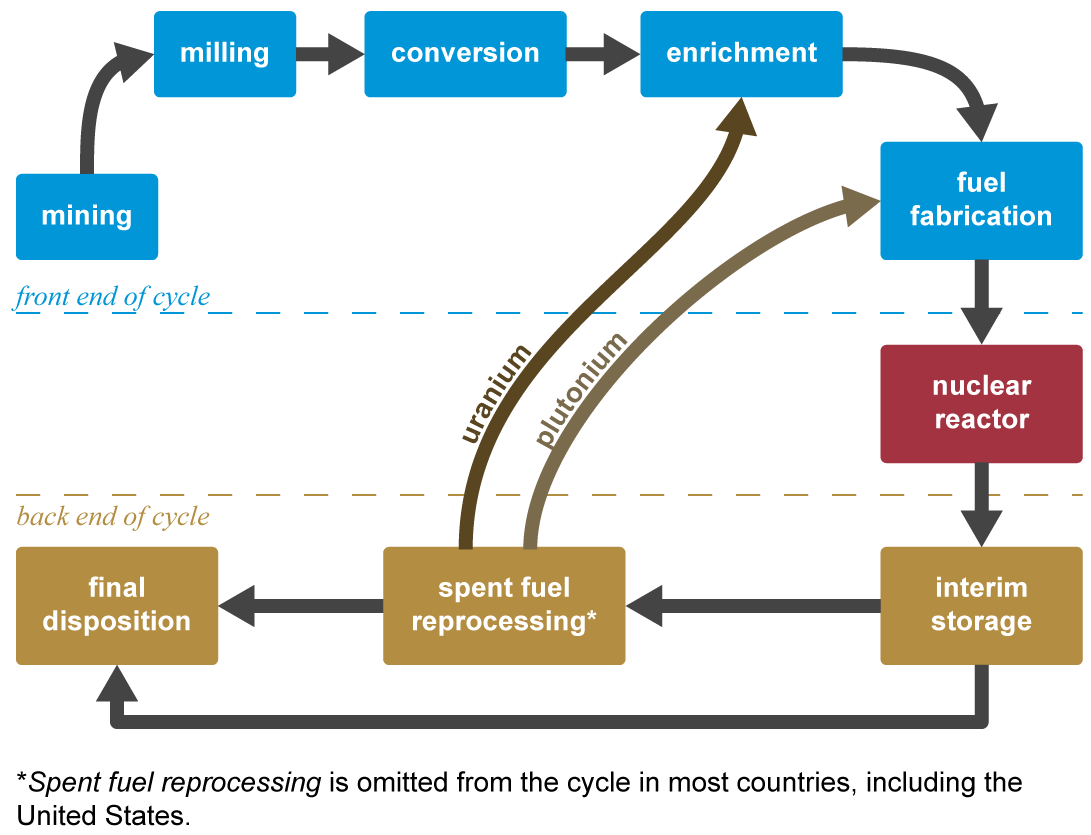
\includegraphics[width=0.75\textwidth]{../images/nuclear_fuel_cycle.png}
      \caption{Source: Penn State Univ. Radiation Science and Engineering Center (public domain)$^{*}$}
      \end{figure}
  \end{frame}

  \begin{frame}
      \frametitle{Not all fuel cycles are made equal, and we want options}
      Concerns about economics, waste generation, proliferation risk, and sustainability motivate the need for fuel cycle options. With metrics like:
        \begin{itemize}%[<+->]
            \item natural resource utilization,
            \item waste mass/volume,
            \item special material quantities,
            \item separative work units,
            \item and energy production,
        \end{itemize}
        we can begin to evaluate the tradeoffs between fuel cycle options.
  \end{frame}

\section{Fuel Cycle Modeling}
  \begin{frame}
    \frametitle{Big questions in fuel cycle modeling}
    Increased computational power and advanced reactors mean more detailed fuel cycle modeling.
    \begin{itemize}
        \item How can we make facility models more accurate?
        \item How can we make transaction models more detailed?
        \item Can we implement nuclear fuel cycle codes to identify realtime diversion or diversion paths?
        \item When do advanced reactor technologies change key metrics we use to evaluate fuel cycles?
    \end{itemize}
  \end{frame}

  \begin{frame}
    \frametitle{We use Cyclus to model fuel cycles}
    \vspace{20pt}
    Cyclus is an open-source agent-based fuel cycle code allowing for detailed facility and transaction modeling \cite{huff_fundamental_2016}.
    \vspace{20pt}
    \begin{figure}
        \centering
        
\includegraphics[width=0.45\textwidth]{../images/cyclus_logo.png}
    \end{figure}

    \vspace{37pt}
    Source: \url{https://github.com/cyclus/cyclus.github.com/blob/source/source/logos/logo2_transp.png}
  \end{frame}

  \begin{frame}
    \frametitle{Cyclus is being used to tackle big questions in fuel cycle modeling}
    \begin{block}{Making facility models more accurate}
        OpenMCyclus \cite{openmcyclus_paper} couples Cyclus with OpenMC to model realtime depletion.
    \end{block}
    \begin{block}{Making transaction models more detailed}
        There is active work to incorporate realistic purchasing agreements and market models into Cyclus.
    \end{block}
    \begin{block}{Identifying realtime diversion or diversion paths}
        CNTAUR \cite{mummah_advanced_2024} and Pyre \cite{westphal_modeling_2019} format outputs in IAEA code 10 format and model real time diversion, respectively.
    \end{block}
    \begin{block}{Finding advanced reactor impacts on the fuel cycle}
        We will talk a little about that today!
    \end{block}
  \end{frame}

  \section{LEU+ to HALEU}
  \begin{frame}
    \frametitle{A mildly provocative question}
    \vspace{-25pt}
    \begin{figure}
        \centering
        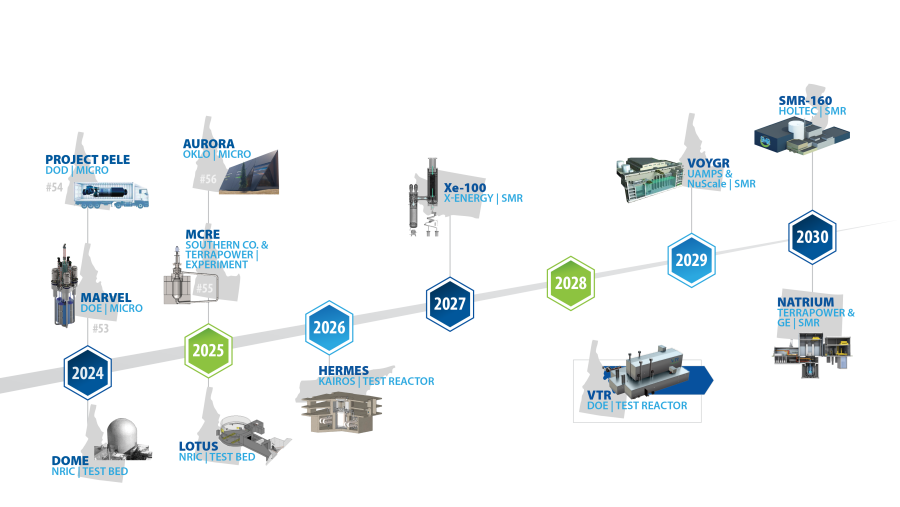
\includegraphics[width=0.98\textwidth]{../images/reactor_timeline.png}
        \caption{Source: \url{inl.gov/nuclear-reactor-sustainment-and-expanded-deployment/}}
    \end{figure}
    \vspace{-8pt}
    What if we can't get HALEU to fuel these advanced reactors?
    Could we use LEU+ in the meantime?
  \end{frame}

  \begin{frame}
    \frametitle{We define the enrichment levels as...}
    These are a mash-up of economic and regulatory definitions.
    \begin{table}[H]
        \centering
        \caption{Enrichment levels and their ranges.}
        \label{tab:enrichment_levels}
        \begin{tabular}{c c}
           \hline
           \textbf{Enrichment Level} & \textbf{Range [\%  $^{235}$U]} \\
           \hline
           Natural & $<$ 0.711 \\
           LEU & 0.711-5 \\
           LEU+ & 5-10 \\
           HALEU & 10-20 \\
           HEU & $\geq$ 20  \\
           \hline
        \end{tabular}
     \end{table}
  \end{frame}

  \begin{frame}
    \frametitle{Our demand for energy is going up}
    \begin{figure}
        \centering
        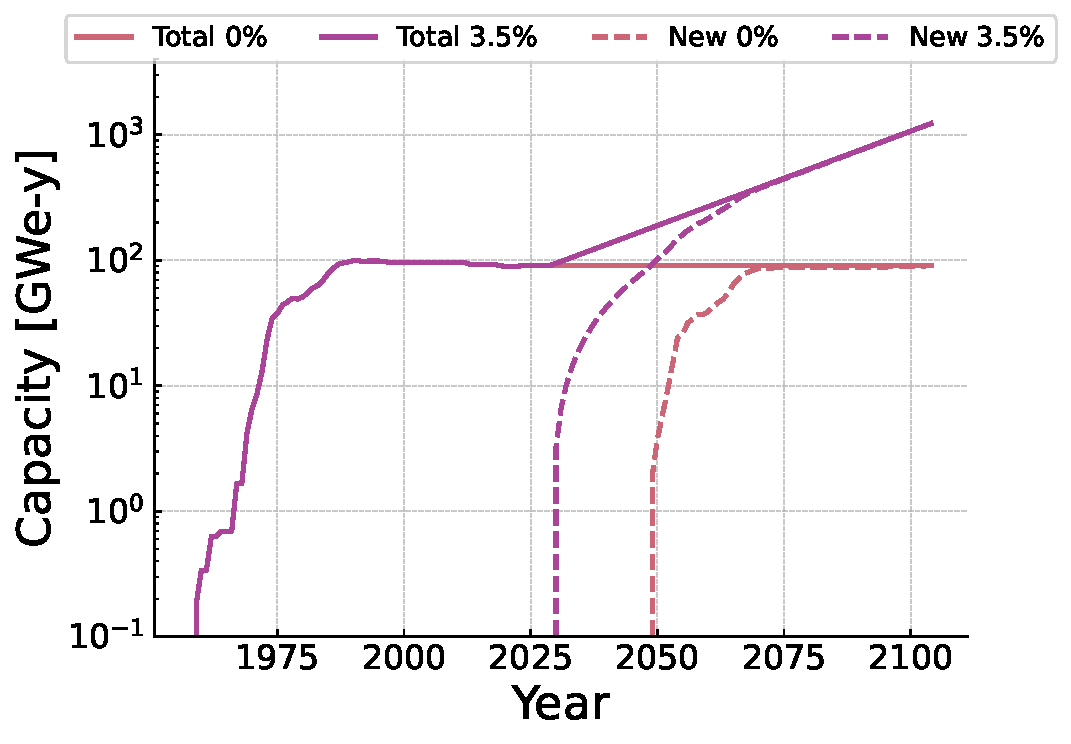
\includegraphics[width=0.85\textwidth]{../images/new_capacity_ng_d2.pdf}
    \end{figure}
  \end{frame}

  \begin{frame}
    \frametitle{Staggering enrichment could give the supply chain time to develop}
    \begin{figure}
        \centering
        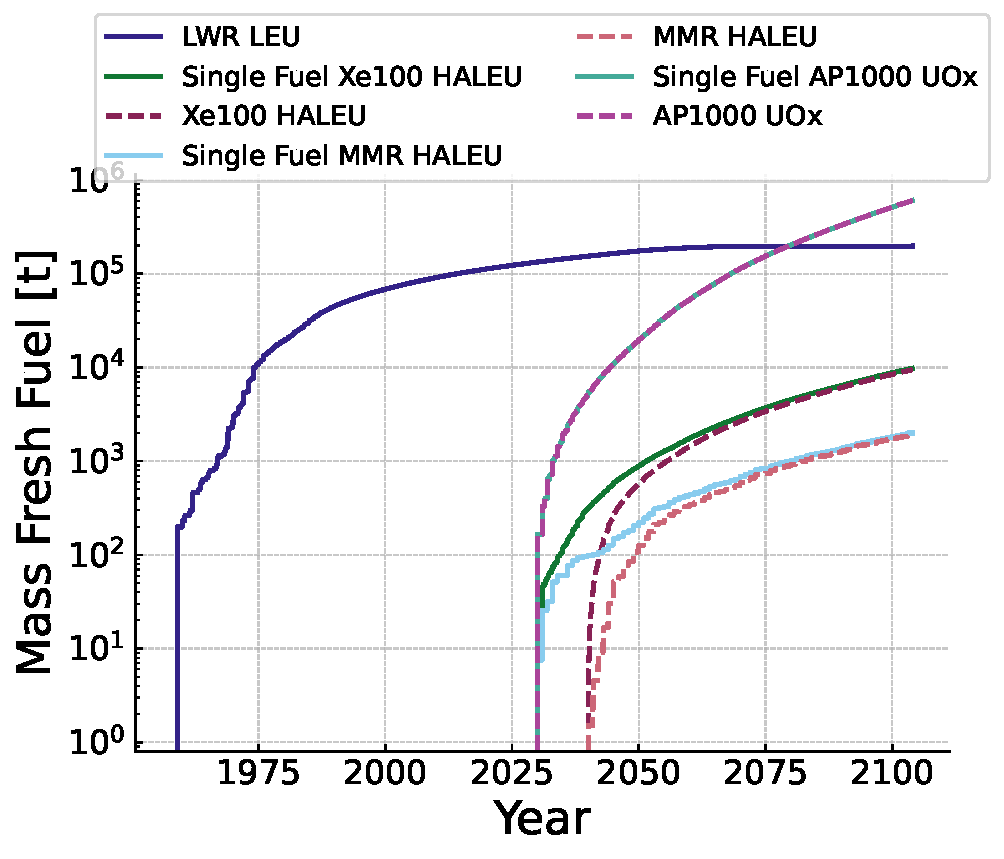
\includegraphics[width=0.75\textwidth]{../images/fresh_fuel.pdf}
    \end{figure}
  \end{frame}

  \begin{frame}
    \frametitle{The difference is on the order of hundreds of tons}
    \begin{figure}
        \centering
        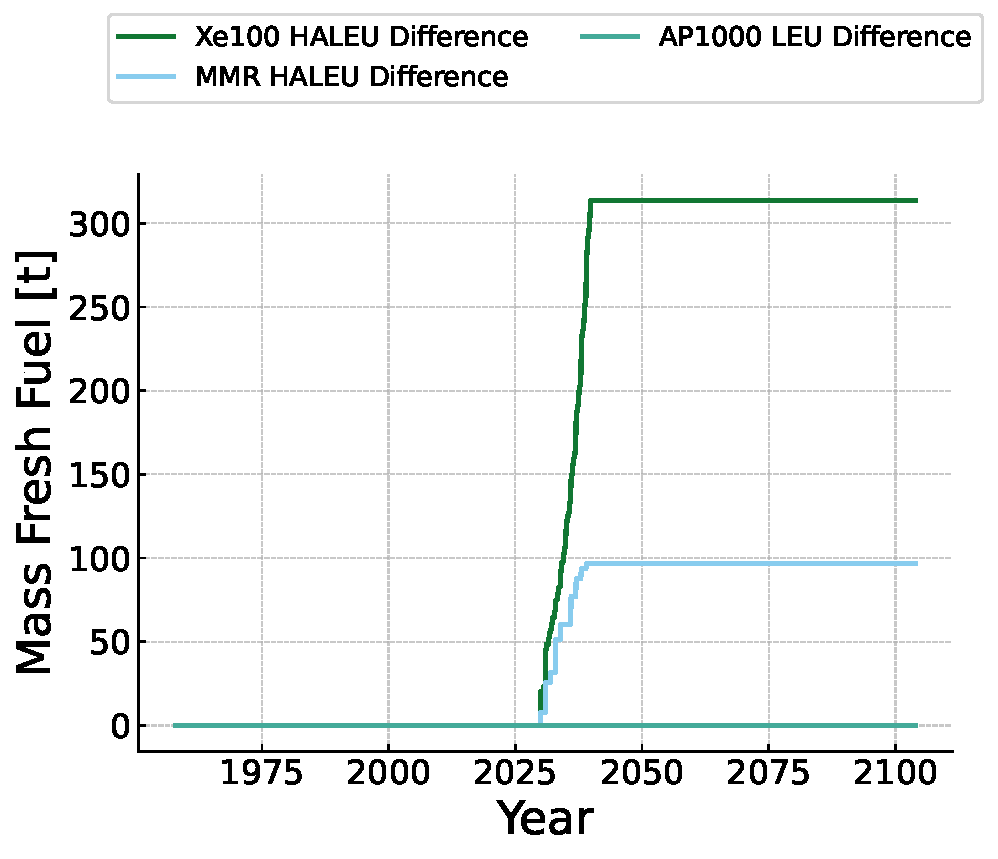
\includegraphics[width=0.75\textwidth]{../images/fresh_fuel_difference.pdf}
    \end{figure}
  \end{frame}


  \section{Conclusion}
  \begin{frame}
      \frametitle{Fuel cycles modeling is useful for enegy planning and safeguards}
      We have covered a tiny fraction of what fuel cycle modeling can do, but there is so much more to do. In our simple case, we transition from LEU+ to HALEU after 10 years of operation.
      \begin{itemize}
          \item For the Xe100 reactors, we need almost 315 less tons of HALEU.
          \item For the MMR reactors, we need almost 97 less tons of HALEU.
      \end{itemize}
      Next we need to characterize what the cost of this transition would be.
  \end{frame}


\begin{frame}
  \frametitle{Acknowledgement}
    This research was performed, in part, using funding received from the DOE
    Office of Nuclear Energy's Nuclear Energy University Program (Project 23-29656
    DE-NE0009390) 'Illuminating Emerging Supply Chain and Waste Management
    Challenges'.


    Thanks to Luke Seifert for his help with running the neutronics models, and thanks to Amanda Bachmann and Zoe Richter for letting me adapt their reactor models for the MMR and Xe100.
\end{frame}




%%--------------------------------%%
%%--------------------------------%%
\begin{frame}[allowframebreaks]
  \frametitle{References}
  \bibliographystyle{plain}
  {\footnotesize \bibliography{../bibliography.bib} }

\end{frame}

\appendix

\begin{frame}
    \frametitle{Know how to code?}
    Consider volunteering as a TA or mentor in the Computational Resource Access NEtwork (CRANE) so we can support more students!
    \begin{figure}
        \centering
        
\includegraphics[width=0.7\textwidth]{../images/CRANE_logo_inverted.png}
    \end{figure}
    Go to our website: \url{https://www.cranephysics.org}
\end{frame}

%%--------------------------------%%


\end{document}



